% !TEX root = ../main.tex
\chapter{Quanto Credit Hedging}\label{ch:quanto}

\begin{sources}
\small
\begin{tabularx}{\linewidth}{@{}l l L@{}}
\toprule
\textbf{Lecture} & \textbf{Speaker} & \textbf{Content}\\
\midrule
2013 L23 & S.~Andreev (Morgan Stanley) & FX spot and forwards, interest-rate parity; the FX betting-game
paradox; sovereign bonds issued in two currencies (Italy) and the credit-spread puzzle; a minimal jump-on-default
FX model; pricing and dynamic hedging of zero-recovery USD/EUR bonds in that model, extension to $R>0$; the
jump-diffusion model left as a final-paper topic; quanto credit default swaps and other applications.\\
\bottomrule
\end{tabularx}

\smallskip
\textbf{Files.} 2013 slides \file{MIT18_S096F13_lecnote23.pdf} (32 slides); accompanying written notes with the
derivations (referenced repeatedly on the slides as ``see class notes'') were not among the materials available
for these notes, so every derivation below is reconstructed from the slides and from the blackboard work described
in the lecture transcript, and re-checked numerically in a Python script written for these notes; reconstructions
are flagged explicitly, and all such numerical checks are marked ``computed for these notes.''
\textbf{Problem sets.} None; the exercises at the end of the chapter are all marked ``not from the course''.
\textbf{Not covered here.} The stochastic-hazard-rate, stochastic-interest-rate, correlated multi-factor version of
the model is only sketched on the last slides (``Real Life''); \cref{ch:hjm} returns to term-structure modelling of
credit.
\end{sources}

\section*{Motivation}
Chapter~\ref{ch:counterparty} showed that a change of numeraire turns a ratio of two traded assets into a
martingale, and listed the FX forward $F_{FX}(t,T)=S_{FX}(t)P^F(t,T)/P^D(t,T)$ as one instance of the pattern
(\cref{ch08:prop-numeraire}). This chapter asks what changes when one of the two ``assets'' can \emph{jump}: a
sovereign issuer defaults, and its currency devalues at the same instant. Two zero-coupon bonds of the same issuer,
one paying 1 USD and one paying 1 EUR, are no longer related by a simple deterministic forward rate, because the
FX rate that converts one payoff into the other is itself correlated with the credit event. Pricing and hedging
one bond with the other -- a \emph{quanto} problem, in the sense that a payoff is being valued in a currency other
than its natural one -- requires modelling the FX jump explicitly.

The chapter builds the smallest possible model that has this feature (a constant-hazard-rate default time with a
deterministic percentage FX jump on default), and carries it through the three-step recipe of
\cref{ch15:sec-onestep}:
\begin{enumerate}[1.]
  \item write the payoffs,
  \item price by risk-neutral expectation and find the replicating
      portfolio,
  \item extract the economic intuition (the sign and size of the ``quanto adjustment'').
\end{enumerate}
The compensator identity used along the way is the jump-process analogue of the risk-neutral drift condition of
\cref{ch15:sec-rn}, and the pricing measure used throughout is exactly the risk-neutral measure $\Q$ of
\cref{ch:bs}; \cref{ch23:sec-numeraire} makes the connection to \cref{ch08:prop-numeraire} precise.

\begin{intuition}[Why symmetric bets are not symmetric]
If I bet you \$100 that a coin lands heads and you bet me 100 EUR that it lands tails, the two bets look
symmetric. They are not, if the coin is Italy defaulting and the EUR devalues whenever it does: winning USD then
happens exactly when EUR is weak, and winning EUR happens exactly when EUR is strong. The currency of the payoff
carries information about the payoff, and a fair price must account for it. This is the whole content of the
chapter, before any formula is written down.
\end{intuition}

\section{FX, interest-rate parity, and the currency of a payoff}\label{ch23:sec-fx}
Write $S_t$ for the spot FX rate USD/EUR, i.e.\ the price in USD of 1 EUR. In the (no-default) Garman--Kohlhagen
model, with domestic (USD) and foreign (EUR) risk-free rates $r_d,r_f$,
\begin{equation}\label{ch23:eq-gk}
  \frac{\dd S_t}{S_t}=(r_d-r_f)\,\dd t+\sigma\,\dd W_t ,\qquad
  S_T=S_0\exp\!\Bigl[(r_d-r_f-\tfrac12\sigma^2)T+\sigma W_T\Bigr],\qquad
  \E[S_T]=S_0e^{(r_d-r_f)T}.
\end{equation}
This is the same lognormal SDE as \cref{ch15:eq-gbm} with $\mu=r_d-r_f$: under $\Q$, a foreign asset earns the
domestic rate once its value is expressed in domestic currency, exactly as a stock earns $r$ under the
risk-neutral measure of \cref{ch15:sec-rn}. The forward FX rate is fixed by no-arbitrage (covered interest-rate
parity), $F(t,T)=S_te^{(r_d-r_f)(T-t)}=\E_t[S_T]$ -- itself an instance of \cref{ch08:prop-numeraire} with
$N_1=1$ (cash) and $N_2=P^D(\cdot,T)$, as recorded in the numeraire table of \cref{ch:counterparty}.

For the rest of the chapter, following the slides, interest rates are set to zero, $r_d=r_f=0$, so that the only
driver of $S_t$ is the credit event: this isolates the ``quanto credit'' effect from the ordinary FX quanto
adjustment of \cref{ch23:eq-gk}, which is unaffected by anything in this chapter and is recovered by simply adding
back $r_d-r_f$ to every drift below.

\begin{finance}[The FX betting game]
Slide 7 poses two \$100-notional bets on whether USD/EUR (currently 1) is above or below 1 in one month. Bet A
pays $\mp\$100$ in USD; Bet B pays $\mp100$ EUR. If the exchange rate is uncorrelated with the outcome the two
bets are worth the same. But if, say, USD/EUR $>1$ (euro strong, dollar weak) exactly in the scenarios where the
bet is lost, then Bet A ($-\$100$ regardless of the rate) is strictly better than Bet B ($-100$ EUR, converted at
an unfavourable rate). Table~\ref{ch23:tab-game} reproduces the slide's numbers: Bet A minus Bet B is always
positive because the loss in Bet B is amplified, and its gain reduced, by exactly the FX move correlated with it. The general
principle: \emph{whenever a payoff and the FX rate used to convert it are correlated, pricing the payoff in the
``wrong'' currency and simply converting at the current spot or forward rate is not valid} -- one must price the
converted payoff directly under a risk-neutral expectation, as done for CDS below.
\end{finance}

\begin{table}[htbp]
\centering
\caption{FX betting game, slide 8: two symmetric-looking \$100/EUR100 bets are worth different amounts once
the payoff currency is correlated with the FX outcome.}\label{ch23:tab-game}
\begin{tabular}{@{}lrrr@{}}
\toprule
Scenario (1 month) & Bet A (USD) & Bet B (EUR, in USD) & A $-$ B\\
\midrule
USD/EUR $=1.25$ & $-100$ & $-125$ & $+25$\\
USD/EUR $=0.75$ & $+100$ & $+75$ & $+25$\\
\bottomrule
\end{tabular}
\end{table}

\section{A reality check: sovereign bonds in two currencies}\label{ch23:sec-italy}
Slides 11--14 use Italy as a running example: a sovereign that issues bonds in EUR and in USD (and other
currencies), with a \emph{cross-default} clause (default on one currency triggers default on all). Two natural
questions: which currency does Italy prefer to borrow in, and which currency do bond investors prefer? The credit
spread (the extra yield over the local risk-free curve) need not be the same in the two currencies, and the slides
show that Italy's EUR and USD five-year credit spreads did in fact move apart during the 2011--2012 sovereign
crisis. Comparing the two spreads directly conflates two different things: the market's view of Italy's
creditworthiness (currency-independent, in a first approximation) and the market's view of what happens to EUR
\emph{if Italy defaults} (which only affects the EUR-denominated bond, since a EUR bond's payoff is naturally
denominated in the currency that would devalue). Section~\ref{ch23:sec-model} builds the smallest model that
captures this second effect, so that the two spreads can be compared on a like-for-like basis.

\subsection{A naive replication attempt, and why it fails}\label{ch23:sec-naive}
Consider two zero-coupon, zero-recovery bonds of the same issuer and maturity $T$: bond $U$ pays 1 USD, bond $E$
pays 1 EUR. With $P_u,P_e$ their prices (in USD and EUR respectively), spot rate $S_t$ and forward rate $F_t$
(USD/EUR, maturity $T$), a naive covered-interest-rate-parity argument suggests buying $100{,}000$ E-bonds, selling
$100{,}000F_t$ U-bonds, and entering a forward to sell $100{,}000$ EUR at $F_t$ (slide 15). If both
bonds survive to $T$, the position pays exactly $0$: the $100{,}000$ EUR received is exchanged at the pre-agreed forward
rate for $100{,}000F_t$ USD, which exactly cancels the short U-bonds. But if the issuer defaults with recovery rate $25\%$
(slide 17), the E-bonds pay $25{,}000$ EUR and the short U-bonds owe $25{,}000F_t$ USD, while the forward contract,
which does not know that the issuer defaulted, still delivers the full $100{,}000$ EUR notional against $100{,}000F_t$ USD.
The strategy is left with a large \emph{unhedged} FX forward position (short $75{,}000$ EUR against $75{,}000F_t$ USD) exactly in the scenario -- default -- in
which EUR is most likely to move sharply (as it did for the Argentine peso in December 2001, slide 18). The naive
strategy is not an arbitrage and is not a valid hedge: the forward is the wrong instrument because it does not
distinguish the default and no-default states. What is needed is a model in which the number of hedging
instruments equals the number of sources of randomness (default timing and the FX jump it triggers) -- a complete
market in the sense of \cref{ch15:sec-onestep} -- so that pricing by replication is again possible.
\section{The minimal jump-on-default FX model}\label{ch23:sec-model}

\subsection{Hazard rate and survival probability}\label{ch23:sec-hazard}
Model the default time $\tau$ of the issuer as the arrival time of the first jump of a Poisson process of constant
intensity $h>0$ (the \emph{hazard rate}): from the perspective of time $t<\tau$,
\begin{equation}\label{ch23:eq-survival}
  \Prob_t(\tau>T)=e^{-h(T-t)},\qquad T\ge t.
\end{equation}
\begin{definition}[Hazard rate]\label{ch23:def-hazard}
$h$ is the instantaneous default intensity: $\Prob_t(\tau\in[t,t+\dd t)\mid\tau>t)=h\,\dd t$.
\end{definition}
\begin{proposition}[Survival probability and default density]\label{ch23:prop-survival}
If $\tau$ has the memoryless survival function \cref{ch23:eq-survival}, then, conditional on $t<\tau$, the density
of $\tau$ at $T>t$ is $\varphi(t,T)=he^{-h(T-t)}$, and the current (\(T\to t\)) default density is $\varphi(t,t)=h$.
\end{proposition}
\begin{proof}
$\Prob_t(\tau\le T)=1-e^{-h(T-t)}$; differentiate in $T$ to get $\varphi(t,T)=he^{-h(T-t)}$; set $T=t$.
\end{proof}
This is exactly the exponential distribution: constant hazard rate $\Leftrightarrow$ $\tau-t\sim\mathrm{Exp}(h)$ given
survival to $t$, the continuous-time analogue of a Poisson arrival process (\cref{ch08:sec-martingale} used the
same intensity idea for the CDS survival measure).

\subsection{FX jump on default}\label{ch23:sec-fxjump}
The model's only new ingredient is that $S_t$ (USD per EUR) jumps by a fixed multiplicative factor at $\tau$:
\begin{equation}\label{ch23:eq-jumpdef}
  S_{\tau}=S_{\tau^-}\,e^{J},\qquad J\in\R,
\end{equation}
so $J<0$ means EUR devalues on default (the Italy/Argentina case) and $J>0$ an appreciation. Let $N_t=\ind_{\{t\ge
\tau\}}$ be the default indicator, a jump process with a single unit jump at $\tau$, $\dd N_t$ the corresponding
point-process differential ($\dd N_t=1$ at $t=\tau$, $0$ elsewhere). Away from the jump, $\log S_t$ is postulated
to drift at some rate $\mu_t$ to be determined:
\begin{equation}\label{ch23:eq-logS}
  \dd\log S_t=\mu_t\,\dd t+J\,\dd N_t .
\end{equation}
No-arbitrage (interest rates being $0$) requires $S_t$ to be a $\Q$-martingale, in particular $\E[S_T]=S_0$ for
every $T$ -- the jump analogue of the risk-neutral drift condition that fixes $\mu=r$ in \cref{ch15:eq-gbm}.

\begin{proposition}[Compensator condition]\label{ch23:prop-compensator}
If $\mu_t=h\bigl(1-e^{J}\bigr)\ind_{\{t<\tau\}}$ in \cref{ch23:eq-logS} (and $\mu_t=0$ once $\tau$ has occurred,
since after default there is nothing left to compensate), then $\E[S_T]=S_0$ for every $T\ge0$.
\end{proposition}
The quantity $h(1-e^J)$ is called the \emph{compensator}: exactly as a Poisson counting process $N_t$ has mean
$ht$ so that $N_t-ht$ is a martingale, here the drift $\mu_t\,\dd t$ must exactly offset, in expectation, the
mean rate of change contributed by the jump term $J\,\dd N_t$, whose expected instantaneous contribution (while
$\tau$ has not yet occurred) is $h\cdot J\,\dd t$ plus a jump-size correction coming from working with $\log S$
rather than $S$ itself; this is made precise in the proof below via It\^o's formula for jump processes.

\begin{lemma}[It\^o's formula for a jump process, reconstruction]\label{ch23:lem-itojump}
Let $X_t$ solve $\dd X_t=\mu_t\,\dd t+J\,\dd N_t$ for a point process $N_t$ with a single jump at $\tau$
(no diffusive part), and let $f\in C^1$. Then
\begin{equation}\label{ch23:eq-itojump}
  \dd f(X_t)=f'(X_t)\,\mu_t\,\dd t+\bigl[f(X_{t^-}+J)-f(X_{t^-})\bigr]\dd N_t .
\end{equation}
\end{lemma}
\begin{proof}
Between jumps $X_t$ is absolutely continuous with $\dot X_t=\mu_t$, so $\dd f(X_t)=f'(X_t)\dot X_t\,\dd t$ by the
ordinary chain rule; at a jump time, $f(X_t)-f(X_{t^-})=f(X_{t^-}+J)-f(X_{t^-})$ by \cref{ch23:eq-jumpdef}-type
jumps of size $J$ in $X$. Summing the continuous drift contribution and the (single) jump contribution gives
\cref{ch23:eq-itojump}. (This is the pure-jump special case of the general jump-diffusion It\^o formula; the
diffusive analogue for Brownian motion is \cref{ch17:thm-ito1}, with the second-derivative term there playing the
role that the finite difference $f(X_{t^-}+J)-f(X_{t^-})$ plays here -- both are ``convexity'' corrections beyond
the naive chain rule, one from quadratic variation, the other from a discrete increment.)
\end{proof}

\begin{proof}[Proof of \cref{ch23:prop-compensator}]
Write $X_t=\log S_t$, so $S_t=e^{X_t}=f(X_t)$ with $f(x)=e^x$. By \cref{ch23:lem-itojump} with $\mu_t$ as in the
statement,
\[
  \dd S_t = S_{t^-}\,h(1-e^J)\ind_{\{t<\tau\}}\,\dd t + S_{t^-}\bigl(e^J-1\bigr)\dd N_t ,
\]
using $f(X_{t^-}+J)-f(X_{t^-})=e^{X_{t^-}}(e^J-1)=S_{t^-}(e^J-1)$. Divide by $S_{t^-}$:
\begin{equation}\label{ch23:eq-dSoverS}
  \frac{\dd S_t}{S_t}=h(1-e^J)\ind_{\{t<\tau\}}\,\dd t+(e^J-1)\,\dd N_t .
\end{equation}
Both terms vanish in expectation instantaneously conditional on survival: on $\{t<\tau\}$, $\E[\dd N_t\mid
\mathcal F_t]=h\,\dd t$, so $\E[\dd S_t/S_t\mid\mathcal F_t,t<\tau]=h(1-e^J)\,\dd t+(e^J-1)h\,\dd t=0$; after
default nothing changes ($\mu_t=0$ and $N_t$ no longer jumps). Hence $S_t$ is a $\Q$-martingale and $\E[S_T]=S_0$.
\end{proof}

\begin{intuition}[Reading the compensator]
If EUR devalues on default ($J<0$, so $e^J<1$), the compensator $h(1-e^J)>0$: between defaults the model must make
EUR \emph{appreciate} against USD, on average, at rate $h(1-e^J)$, precisely so that the (rare, large, negative)
jump at default leaves the unconditional mean unchanged. This upward drift before default is a purely technical
artefact of no-arbitrage in a jump model, not a forecast: it is the exact analogue of the fact that a stock with a
possible downward jump (bankruptcy) must drift upward the rest of the time to keep $\E[S_T]$ fixed at the forward
level, a fact well known from equity jump-diffusion models.
\end{intuition}

\subsection{Explicit solution for \texorpdfstring{$S_t$}{S\_t}}\label{ch23:sec-explicit}
\begin{proposition}[Path of the FX rate]\label{ch23:prop-Spath}
Under \cref{ch23:eq-logS} with the compensator drift of \cref{ch23:prop-compensator},
\begin{equation}\label{ch23:eq-Spath}
  S_T=S_0\exp\Bigl[h\bigl(1-e^J\bigr)(T\wedge\tau)+J\,\ind_{\{\tau\le T\}}\Bigr],
  \qquad T\wedge\tau=\min(T,\tau).
\end{equation}
Equivalently: if $\tau>T$, $S_T=S_0\exp[h(1-e^J)T]$ (pure drift); if $\tau\le T$, $S_T=S_0\exp[h(1-e^J)\tau+J]$
(drift up to default, then the jump).
\end{proposition}
\begin{proof}
Integrate \cref{ch23:eq-logS}: $\log S_T-\log S_0=\int_0^Th(1-e^J)\ind_{\{t<\tau\}}\dd t+J\int_0^T\dd N_t$. The first
integral runs only while $t<\tau$, i.e.\ up to $T\wedge\tau$, contributing $h(1-e^J)(T\wedge\tau)$; the second is
$J$ if a jump occurred by $T$ ($\tau\le T$) and $0$ otherwise. Exponentiate.
\end{proof}

\begin{example}[Numerical check of the martingale property]\label{ch23:ex-mc}
Take $h=0.05$, $J=-0.30$ (a $30\%$ devaluation on default, roughly the order of magnitude of the Argentine peso
move of slide 18), $T=3$, $S_0=1$. Monte Carlo with $6\times10^6$ paths of $\tau\sim\mathrm{Exp}(h)$ and
\cref{ch23:eq-Spath} gives $\widehat\E[S_T]=0.99997$, matching the required value $S_0=1$ to four significant
figures (computed for these notes; ). The exact identity
$\E[S_T]=1$ can also be checked analytically by splitting the expectation on $\{\tau>T\}$ and $\{\tau\le T\}$ and
integrating $\varphi(0,\tau)=he^{-h\tau}$ against \cref{ch23:eq-Spath}; both routes agree.
\end{example}
\section{Pricing and hedging zero-recovery bonds}\label{ch23:sec-pricing}
Consider zero-coupon, zero-recovery bonds of maturity $T$ from the same issuer: $U$ pays 1 USD at $T$ if
$\tau>T$ (and $0$ otherwise); $E$ pays 1 EUR at $T$ under the same condition. Both are priced, in USD, by
risk-neutral expectation (interest rates $0$, so the money-market numeraire is $\beta(t)\equiv1$, as in
\cref{ch08:sec-martingale}):
\begin{equation}\label{ch23:eq-Pu}
  P_u(0,T)=\E\bigl[\ind_{\{\tau>T\}}\bigr]=\Prob(\tau>T)=e^{-hT},
\end{equation}
by \cref{ch23:eq-survival}, exactly as in \cref{ch15:sec-rn}: the price is the expected discounted payoff. For the
EUR bond, the USD-payoff is $S_T\ind_{\{\tau>T\}}$ (converting the 1 EUR payoff at the terminal FX rate), so
\begin{equation}\label{ch23:eq-Pe-setup}
  P_e(0,T)=\E\bigl[S_T\,\ind_{\{\tau>T\}}\bigr].
\end{equation}

\begin{proposition}[Zero-recovery bond prices]\label{ch23:prop-bondprices}
\begin{equation}\label{ch23:eq-bondprices}
  P_u(0,T)=e^{-hT},\qquad\qquad P_e(0,T)=S_0\,e^{-h e^{J}T}.
\end{equation}
\end{proposition}
\begin{proof}
$P_u$ is \cref{ch23:eq-Pu}. For $P_e$, on $\{\tau>T\}$, \cref{ch23:eq-Spath} gives $S_T=S_0e^{h(1-e^J)T}$ (a constant,
not random, given survival), so
\[
  P_e(0,T)=S_0e^{h(1-e^J)T}\,\Prob(\tau>T)=S_0e^{h(1-e^J)T}e^{-hT}=S_0\,e^{hT(1-e^J)-hT}=S_0\,e^{-h e^JT}.
  \qedhere
\]
\end{proof}
Formula \eqref{ch23:eq-bondprices} was checked numerically for these notes: with $h=0.05$, $J=-0.30$, $T=3$,
$S_0=1$, \cref{ch23:eq-bondprices} gives $P_u=0.86071$, $P_e=0.89483$, against Monte Carlo estimates $0.86059$ and
$0.89470$ from $6\times10^6$ paths -- agreement to three decimals.

\begin{intuition}[Reading $P_e$]
$P_e/S_0=e^{-h e^JT}$ rather than $e^{-hT}$: the EUR bond is priced with an \emph{effective hazard rate}
$h_{\mathrm{eff}}=he^J$ once expressed in USD. If EUR devalues on default ($J<0$, $e^J<1$), $h_{\mathrm{eff}}<h$
and $P_e/S_0>P_u$: in USD terms the EUR bond looks \emph{less} risky than the USD bond of the same issuer, because
its payoff is worth relatively little exactly in the states where default has happened -- the market has less to
lose, in USD, from that scenario. This is the quanto adjustment for credit: the raw survival probability $e^{-hT}$
is corrected by $e^J$ to account for the correlation between the default event and the currency of the payoff. It
matches the qualitative content of the Italy example of \cref{ch23:sec-italy}: everything else equal, a devaluing
local-currency bond should trade with a \emph{lower} USD-equivalent implied hazard rate than the hard-currency
bond of the same issuer -- exactly the pattern the slides point to (EUR spread below USD spread once basis-adjusted).
\end{intuition}

\subsection{The replicating portfolio}\label{ch23:sec-replicate}
Sell one $U$ bond and buy $N_E(t)=P_u(t,T)/P_e(t,T)$ $E$-bonds so that the portfolio costs $0$ at every rebalancing
date; by \cref{ch23:eq-bondprices} (evaluated at $t$ instead of $0$, since \cref{ch23:prop-bondprices} only uses
the survival probability from $t$ to $T$, hence holds for any $t<\tau$),
\begin{equation}\label{ch23:eq-hedgeratio}
  N_E(t)=\frac{P_u(t,T)}{P_e(t,T)}=\frac{e^{-h(T-t)}}{S_te^{-he^J(T-t)}}=\frac{1}{S_t}\exp\bigl[h(T-t)(e^J-1)\bigr].
\end{equation}
\begin{proposition}[The portfolio is a hedge]\label{ch23:prop-replicate}
The portfolio $\Pi_t=-P_u(t,T)+N_E(t)P_e(t,T)\equiv0$ for every $t<\tau$; if default occurs, both bonds are worth
$0$ (zero recovery) so $\Pi_\tau=0$ as well. Hence the portfolio replicates the (trivial) zero payoff in every
state, and the hedge ratio \cref{ch23:eq-hedgeratio} is the unique arbitrage-free hedge of one bond against the
other.
\end{proposition}
\begin{proof}
$\Pi_t=-P_u(t,T)+N_E(t)P_e(t,T)=-P_u(t,T)+P_u(t,T)=0$ by construction of $N_E(t)$, for every $t<\tau$ (not only
$t=0$), because \cref{ch23:eq-bondprices} depends on $t$ only through the remaining maturity $T-t$ and through
$S_t$, and $N_E(t)$ was defined by dividing them; the $S_t$ dependence cancels exactly between $P_e(t,T)$'s
explicit $S_t$ factor and $N_E(t)$'s $1/S_t$ factor. At default both bonds default to $0$ recovery, so $\Pi_\tau=0$
trivially. What makes this a genuine hedge, and not a tautology, is that the rebalancing is \emph{self-financing}:
before default $\dd\log P_u(t,T)=h\,\dd t$ and $\dd\log P_e(t,T)=\dd\log S_t+he^J\dd t=h\,\dd t$ (by
\cref{ch23:eq-logS} with the compensator drift), and both bonds jump to $0$ at $\tau$, so
$\dd P_u/P_{u}=\dd P_e/P_{e}=h\,\dd t-\dd N_t$. Hence $-\dd P_u+N_E\,\dd P_e=0$: the gains of the position are
identically zero, and the $N_E(t)$ $E$-bonds, rebalanced at no cost, replicate one $U$-bond.
\end{proof}
This was checked numerically: with the parameters of \cref{ch23:ex-mc} and $T=3$, $N_E(0)=0.96187$
($=e^{h T(e^J-1)}$ since $S_0=1$); stepping $\Delta t=0.4$ forward with no default, both $P_u$ and $N_E(t)P_e(t,T)$
were recomputed from \cref{ch23:eq-bondprices}--\eqref{ch23:eq-hedgeratio} and agreed to machine precision, confirming \cref{ch23:prop-replicate} directly rather than only through the algebraic
cancellation in the proof.

\begin{remark}[Why this is harder than static replication]\label{ch23:rem-dynamic}
$N_E(t)$ depends on $t$ (through the remaining maturity) and on $S_t$ (through the $1/S_t$ factor): the hedge must
be \emph{continuously rebalanced}, unlike a naive static forward hedge. It also depends on $h$ and $J$: how many
EUR bonds are needed to hedge one USD bond depends on both the issuer's credit riskiness and the size of the FX
move it would trigger, not only on the current spot or forward FX rate. This is the chapter's central point: an
FX forward, which prices only the correlation-free part of the FX/credit relationship, cannot replicate a
credit-quanto payoff; only a model with an explicit joint dynamics for $(\tau,S)$ can.
\end{remark}

\section{Non-zero recovery}\label{ch23:sec-recovery}
If the recovery rate is $R\in(0,1)$, the bond payoffs at $T$ become $1$ (USD, resp.\ EUR) if $\tau>T$ and $R$ if
$\tau\le T$.
\begin{proposition}[Bond prices with recovery, reconstruction]\label{ch23:prop-recovery}
\begin{equation}\label{ch23:eq-recovery}
  P_u^R(0,T)=R+(1-R)e^{-hT},\qquad\qquad P_e^R(0,T)=S_0\Bigl[R+(1-R)e^{-he^JT}\Bigr].
\end{equation}
\end{proposition}
\begin{proof}
$P_u^R(0,T)=\E[\ind_{\{\tau>T\}}+R\ind_{\{\tau\le T\}}]=\Prob(\tau>T)+R\Prob(\tau\le T)=e^{-hT}+R(1-e^{-hT})$, which
rearranges to the stated form. For $P_e^R(0,T)/S_0=\E[e^{X_T}\ind_{\{\tau>T\}}+Re^{X_T}\ind_{\{\tau\le T\}}]$ with
$X_T=\log(S_T/S_0)$ from \cref{ch23:eq-Spath}: the first term is $P_e(0,T)/S_0=e^{-he^JT}$ by
\cref{ch23:prop-bondprices}. The second term integrates over the default density $\varphi(0,\tau)=he^{-h\tau}$ of
\cref{ch23:prop-survival}, using $X_T=h(1-e^J)\tau+J$ on $\{\tau\le T\}$:
\[
  R\int_0^Te^{h(1-e^J)\tau+J}\,he^{-h\tau}\,\dd\tau
  =Rhe^J\!\int_0^Te^{-he^J\tau}\,\dd\tau
  =Rhe^J\cdot\frac{1-e^{-he^JT}}{he^J}
  =R\bigl(1-e^{-he^JT}\bigr).
\]
Adding the two terms, $P_e^R(0,T)/S_0=e^{-he^JT}+R(1-e^{-he^JT})=R+(1-R)e^{-he^JT}$.
\end{proof}
The two formulas in \cref{ch23:eq-recovery} are strikingly parallel: each is $R+(1-R)$ times the corresponding
zero-recovery survival probability, with $h$ replaced by $he^J$ in the EUR case. This was checked both by
numerical quadrature of the integral above and by Monte Carlo (parameters as in \cref{ch23:ex-mc}, $R=0.25$):
$P_u^R=0.89553$ (formula) vs.\ $0.89544$ (MC), $P_e^R=0.92112$ (formula, matching the quadrature to 6 digits) vs.\
$0.92102$ (MC).

\begin{remark}[Exact replication is lost]\label{ch23:rem-Rgt0}
With $R>0$ the ratio $P_u^R(t,T)/P_e^R(t,T)$ no longer has the clean multiplicative form of
\cref{ch23:eq-hedgeratio} (the $R$ and $(1-R)e^{-h(\cdot)T}$ terms scale differently with $S_t$ and with $T-t$), so
the zero-cost ratio $P_u^R/P_e^R$ no longer matches the two bonds' jumps at default, and a portfolio of the two bonds
alone is no longer a hedge. The model is still complete (one jump, one risky hedge instrument): holding
$N_E(t)=\Delta P_u^R/\Delta P_e^R$ $E$-bonds, the ratio of the jumps at default
($\Delta P_u^R=R-P_u^R(t,T)$, $\Delta P_e^R=RS_te^J-P_e^R(t,T)$), plus the USD cash needed to match the value,
replicates the $U$-bond, because both prices are $\Q$-martingales and their drifts are fixed by their jumps
(reconstruction, not in the slides). The slides stop here (``even in such a simple model,
hedging is not trivial''); \cref{ch23:sec-jumpdiffusion} sketches the further step (adding a diffusive component)
proposed as a final-project topic.
\end{remark}

\begin{figure}[htbp]
\centering
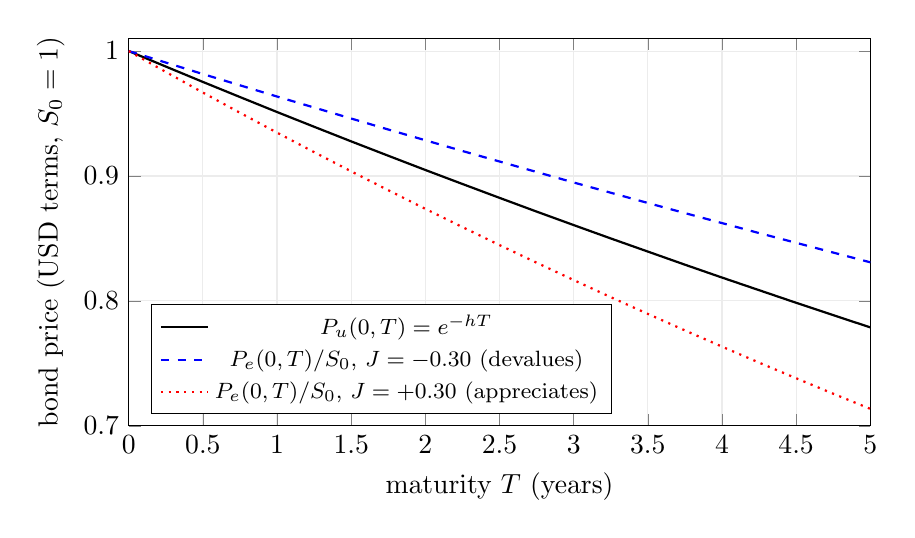
\begin{tikzpicture}
\begin{axis}[
  width=11cm,height=6.5cm,
  xlabel={maturity $T$ (years)}, ylabel={bond price (USD terms, $S_0=1$)},
  xmin=0,xmax=5, ymin=0.7,ymax=1.01,
  legend pos=south west, legend style={font=\footnotesize},
  grid=both, grid style={gray!15},
]
\addplot[thick,black] coordinates {
(0.00,1.0000) (0.25,0.9876) (0.50,0.9753) (0.75,0.9632) (1.00,0.9512) (1.25,0.9394) (1.50,0.9277)
(1.75,0.9162) (2.00,0.9048) (2.25,0.8936) (2.50,0.8825) (2.75,0.8715) (3.00,0.8607) (3.25,0.8500)
(3.50,0.8395) (3.75,0.8290) (4.00,0.8187) (4.25,0.8086) (4.50,0.7985) (4.75,0.7886) (5.00,0.7788)};
\addlegendentry{$P_u(0,T)=e^{-hT}$}
\addplot[thick,blue,dashed] coordinates {
(0.00,1.0000) (0.25,0.9908) (0.50,0.9816) (0.75,0.9726) (1.00,0.9636) (1.25,0.9548) (1.50,0.9460)
(1.75,0.9372) (2.00,0.9286) (2.25,0.9200) (2.50,0.9116) (2.75,0.9032) (3.00,0.8948) (3.25,0.8866)
(3.50,0.8784) (3.75,0.8703) (4.00,0.8623) (4.25,0.8543) (4.50,0.8465) (4.75,0.8387) (5.00,0.8309)};
\addlegendentry{$P_e(0,T)/S_0$, $J=-0.30$ (devalues)}
\addplot[thick,red,dotted] coordinates {
(0.00,1.0000) (0.25,0.9833) (0.50,0.9668) (0.75,0.9506) (1.00,0.9347) (1.25,0.9191) (1.50,0.9037)
(1.75,0.8886) (2.00,0.8737) (2.25,0.8591) (2.50,0.8447) (2.75,0.8306) (3.00,0.8167) (3.25,0.8030)
(3.50,0.7896) (3.75,0.7764) (4.00,0.7634) (4.25,0.7506) (4.50,0.7381) (4.75,0.7257) (5.00,0.7136)};
\addlegendentry{$P_e(0,T)/S_0$, $J=+0.30$ (appreciates)}
\end{axis}
\end{tikzpicture}
\caption{Zero-recovery bond prices \eqref{ch23:eq-bondprices}, $h=0.05$. A currency that devalues on default
($J<0$) makes the local-currency bond look \emph{less} risky in hard-currency terms ($P_e>P_u$); a currency that
appreciates on default ($J>0$, unusual but not impossible for a safe-haven funding currency) makes it look
\emph{more} risky ($P_e<P_u$). Coordinates computed for these notes in Python.}\label{ch23:fig-bonds}
\end{figure}
\section{Change of numeraire view}\label{ch23:sec-numeraire}
The pricing formula \eqref{ch23:eq-Pe-setup}, $P_e(0,T)/S_0=\E[e^{X_T}\ind_{\{\tau>T\}}]$, can be read as a change
of numeraire in the sense of \cref{ch08:prop-numeraire}. Take $N_1(t)=S_t$ (EUR converted to USD, a traded USD
asset since interest rates are $0$) and $N_2(t)=1$ (USD cash). By \cref{ch08:prop-numeraire},
\[
  \E_0^{\Q}\bigl[Y_T\bigr]=\frac{N_1(0)}{N_2(0)}\,\E_0^{\Q_{S}}\!\left[Y_T\,\frac{N_2(T)}{N_1(T)}\right]
  \quad\Longrightarrow\quad
  \E_0^{\Q}\bigl[S_TY_T\bigr]=S_0\,\E_0^{\Q_S}[Y_T],
\]
where $\Q_S$ is the measure associated with numeraire $S$ (the ``EUR risk-neutral measure expressed in USD units,''
by the Radon--Nikod\'ym derivative $\dd\Q_S/\dd\Q|_{\mathcal F_T}=S_T/S_0$, since $S_t/1$ is itself the
$\Q$-martingale that must be used in \cref{ch08:prop-numeraire}). With $Y_T=\ind_{\{\tau>T\}}$,
\begin{equation}\label{ch23:eq-numeraire-view}
  P_e(0,T)=S_0\,\Prob_0^{\Q}(\tau>T)\Big|_{\text{naive}}\ \ne\ P_e(0,T)=S_0\,\Q_S(\tau>T),
\end{equation}
and \cref{ch23:prop-bondprices} says precisely that $\Q_S(\tau>T)=e^{-he^JT}\ne e^{-hT}=\Q(\tau>T)$: default is
\emph{less} likely under the EUR-numeraire measure $\Q_S$ than under $\Q$ when $J<0$ (EUR weakens on default) --
because $\Q_S$ tilts probability towards paths on which $S_T$ is large, i.e.\ towards the surviving, no-jump
scenario. This is exactly the same mechanism as the FX-forward row of the numeraire table in
\cref{ch08:sec-martingale}, $F_{FX}(t,T)=S_{FX}(t)P^F(t,T)/P^D(t,T)$, except that here the ``foreign bond'' $P^F$ is
itself default-risky and its numeraire property breaks down exactly at $\tau$ (it is only a valid numeraire, i.e.\
strictly positive, on $\{t<\tau\}$) -- the same obstruction \cref{ch08:sec-martingale} met when trying to use the
risky annuity $\tilde A_j$ as a numeraire for the CDS survival measure, and resolved there the same way: work with
$\ind_{\{t<\tau\}}$ times the relevant traded quantity, which \emph{is} a genuine $\Q$-martingale even though the
numeraire itself is not always positive.

\begin{intuition}[Quanto adjustment = change of measure]
Every ``quanto adjustment'' in this course -- FX quanto options, quanto CDS here -- is a change of numeraire from
the natural currency's risk-neutral measure to the payoff currency's risk-neutral measure. When the underlying
(here, the default indicator) is independent of the FX rate, the two measures agree and quanto pricing reduces to
discounting by the forward FX rate. When they are correlated (through the jump $J$), the Radon--Nikod\'ym
derivative $S_T/S_0$ tilts the default probability, and no amount of forward-FX-based reasoning like
\cref{ch23:sec-naive} can substitute for computing the expectation under the correct measure.
\end{intuition}

\section{Quanto credit default swaps and other applications}\label{ch23:sec-quanto-cds}
A credit default swap (CDS) is a bilateral insurance contract on the issuer's default: the protection buyer pays a
periodic spread (the premium leg) until default or maturity, and receives $1-R$ per unit notional from the
protection seller if default occurs (the protection leg). A \emph{quanto CDS} is a CDS whose notional and premium
are denominated in a currency different from the reference obligation's natural currency -- e.g.\ a CDS on Brazil
denominated in Brazilian reais rather than in USD. Exactly the mechanism of this chapter applies: if the reference
entity's local currency devalues on default (as is typical for a sovereign or an issuer whose revenues are tied to
its home currency), then a protection payment fixed in local currency is worth less, in hard-currency terms,
precisely when it is needed -- the quanto CDS spread must be adjusted relative to the hard-currency CDS spread by
a factor analogous to $e^J$ in \cref{ch23:eq-bondprices}, and the correct hedge ratio between the two currencies'
CDS again requires the jump-on-default FX model rather than a simple FX forward. Historically, quanto CDS were
often priced by simply converting the hard-currency CDS spread at the current or forward FX rate, ignoring the
correlation; this reproduces neither the observed market prices nor a valid hedge ratio, which is exactly why a
model with the jump feature became necessary in practice.

\begin{casestudy}[Sovereign quanto CDS baskets]
During the European sovereign crisis (2010--2012), USD- and EUR-denominated CDS on peripheral euro-area sovereigns
(Italy, Spain, Portugal) diverged, giving rise to an actively quoted ``quanto'' basis. Market participants used
models of the type developed here (often with stochastic hazard rates and a jump-diffusion FX process, as sketched
in \cref{ch23:sec-jumpdiffusion}) to convert between the USD and EUR curves and to size cross-currency hedges,
essentially betting on how far the euro would fall if a member state defaulted or exited the currency union.
\end{casestudy}

\section{Towards a more realistic model}\label{ch23:sec-jumpdiffusion}
The pure-jump FX process of \cref{ch23:eq-dSoverS} has no day-to-day volatility except at $\tau$: a natural next
step (posed on the slides as a final-project topic) is to add a diffusive component,
\begin{equation}\label{ch23:eq-jumpdiffusion}
  \frac{\dd S_t}{S_t}=h\bigl(1-e^J\bigr)\ind_{\{t<\tau\}}\,\dd t+\bigl(e^J-1\bigr)\dd N_t+\sigma\,\dd W_t,
\end{equation}
a genuine jump-diffusion in the sense of \cref{ch17:sec-lemma} plus \cref{ch23:sec-fxjump} combined: away from
$\tau$, $S_t$ behaves like the ordinary geometric Brownian motion of \cref{ch23:eq-gk}; at $\tau$, it also jumps by
$e^J$. Pricing bonds in this model requires It\^o's formula with \emph{both} a diffusive and a jump term (the
sum of the Brownian second-derivative correction of \cref{ch17:thm-ito2} and the finite-difference jump correction
of \cref{ch23:lem-itojump}), and hedging now needs (at least) two instruments -- an FX forward for the diffusive
risk and a position sensitive to the jump (e.g.\ a short-dated deep out-of-the-money FX option, or the bonds
themselves) -- since the model has two independent sources of randomness ($W$ and $N$), matching the ``number of
hedging instruments = number of stochastic sources'' completeness criterion of \cref{ch15:sec-onestep}. Once a
closed-form or PDE solution is obtained, it can (and should) be checked against a Monte Carlo simulation that
simulates $\tau$, $W$, and hence $S_T$, jointly, exactly as done at smaller scale in \cref{ch23:ex-mc}. In the more
realistic desk models this course only sketches, both the hazard rate and interest rates are themselves stochastic
and correlated with FX (``Real Life'', slide 29); \cref{ch:hjm} develops the term-structure machinery needed to
make hazard rates stochastic in a no-arbitrage way, and correlating them with FX and with rates is a natural
(unaddressed here) extension of the multi-factor models built there. Because defaults are rare, naive Monte Carlo
is inefficient (most paths never see a jump); practitioners typically integrate the payoff analytically over the
default-time density $\varphi(0,\tau)$ (as done by hand in \cref{ch23:prop-recovery}) and simulate only the
diffusive factors (FX, rates, hazard-rate level) by Monte Carlo, mixing the two techniques.

\section{Girsanov and the diffusive quanto adjustment}\label{ch23:sec-girsanov}
It is worth relating \cref{ch23:eq-jumpdiffusion} back to the purely diffusive quanto adjustment familiar from FX
options (not covered in the 2013 lecture, but a standard consequence of \cref{ch17:sec-girsanov}). If a foreign
asset $V_t$ (say, a EUR equity index) follows a geometric Brownian motion under
the foreign risk-neutral measure $\Q^F$ and the FX rate $S_t$ one under the domestic measure $\Q^D$,
\[
  \frac{\dd V_t}{V_t}=r_f\,\dd t+\sigma_V\,\dd W_t^F,\qquad
  \frac{\dd S_t}{S_t}=(r_d-r_f)\,\dd t+\sigma_S\,\dd \widetilde W_t^D,\qquad
  \dd W^F\,\dd\widetilde W^D=\rho\,\dd t,
\]
then pricing a USD-denominated (\emph{quantoed}) payoff on $V_T$ requires switching from $\Q^F$ to the domestic
measure $\Q^D$. Girsanov's theorem (\cref{ch17:sec-girsanov}) says this changes the drift of $V$ by
$-\rho\sigma_V\sigma_S$: under $\Q^D$, $V$ grows at $r_f-\rho\sigma_V\sigma_S$ rather than at $r_f$. This is the
textbook ``quanto drift adjustment,'' and it is the diffusive sibling of the jump compensator
\cref{ch23:prop-compensator}: in both cases, expressing a foreign payoff in domestic currency under the correlated
FX process shifts the effective drift of the payoff by an amount proportional to the FX/payoff correlation --
$-\rho\sigma_V\sigma_S$ in the Brownian case, $h(e^J-1)$ (via the jump-driven change of measure of
\cref{ch23:sec-numeraire}) in the jump case. \cref{ch23:eq-jumpdiffusion} simply has both effects at once.

\begin{keyformulas}
\begin{align*}
&\text{Survival:} && \Prob_t(\tau>T)=e^{-h(T-t)}\quad\text{(\cref{ch23:eq-survival})}\\
&\text{FX dynamics:} && \dd S_t/S_t=h(1-e^J)\ind_{\{t<\tau\}}\dd t+(e^J-1)\dd N_t\quad\text{(\cref{ch23:eq-dSoverS})}\\
&\text{Zero-recovery bonds:} && P_u(0,T)=e^{-hT},\quad P_e(0,T)=S_0\,e^{-he^JT}\quad\text{(\cref{ch23:eq-bondprices})}\\
&\text{Hedge ratio:} && N_E(t)=\tfrac1{S_t}\exp[h(T-t)(e^J-1)]\quad\text{(\cref{ch23:eq-hedgeratio})}\\
&\text{Bonds, recovery $R$:} && P_u^R(0,T)=R+(1-R)e^{-hT}\\
& && P_e^R(0,T)=S_0[R+(1-R)e^{-he^JT}]\quad\text{(\cref{ch23:eq-recovery})}
\end{align*}
\end{keyformulas}

\section*{Exercises}
\addcontentsline{toc}{section}{Exercises}
\begin{exercise}[No devaluation, not from the course]\label{ch23:ex-J0}
Show that if $J=0$ (no FX jump on default), \cref{ch23:eq-bondprices} collapses to $P_u(0,T)=P_e(0,T)/S_0=e^{-hT}$
and the hedge ratio \eqref{ch23:eq-hedgeratio} collapses to $N_E(t)=1/S_t$ -- the ordinary FX conversion, with no
quanto correction, as expected when default carries no currency information.
\end{exercise}

\begin{exercise}[Sign of the quanto adjustment, not from the course]\label{ch23:ex-sign}
Using \cref{ch23:eq-bondprices}, show that $P_e(0,T)/S_0>P_u(0,T)$ if and only if $J<0$ (devaluation on default),
for every $h>0,T>0$. Interpret: does a devaluing local currency make the local-currency bond, expressed in hard
currency, look safer or riskier than the equivalent hard-currency bond of the same issuer?
\end{exercise}

\begin{exercise}[Small-jump limit, not from the course]\label{ch23:ex-small}
Expand $P_e(0,T)$ of \cref{ch23:eq-bondprices} to first order in $J$ around $J=0$ and show
$P_e(0,T)\approx S_0e^{-hT}(1-hTJ)$. Compare with $P_u(0,T)=e^{-hT}$ and give a one-line rule of thumb for the
size of the quanto adjustment to the credit spread (defined as $-\tfrac1T\log P$) when $J$ is small.
\end{exercise}

\begin{exercise}[Recovery limits, not from the course]\label{ch23:ex-recovery-limits}
Check that \cref{ch23:eq-recovery} reduces to \cref{ch23:eq-bondprices} when $R=0$, and to $P_u^R=P_e^R/S_0=1$ for
every $T$ when $R=1$ (a bond that always pays its notional regardless of default is riskless). Explain why the
second limit no longer depends on $h$ or $J$.
\end{exercise}

\begin{exercise}[Compensator with two jump sizes, not from the course]\label{ch23:ex-twojumps}
Suppose $S_t$ can jump on default to either $S_{\tau^-}e^{J_1}$ (probability $p$) or $S_{\tau^-}e^{J_2}$
(probability $1-p$), independently drawn at $\tau$. Redo the proof of \cref{ch23:prop-compensator} to find the
compensator drift $\mu_t$ that keeps $S_t$ a $\Q$-martingale, and check that it reduces to
\cref{ch23:prop-compensator} when $p=1$.
\end{exercise}

\begin{exercise}[Monte Carlo verification, not from the course]\label{ch23:ex-mc-exercise}
Reproduce \cref{ch23:ex-mc} in Python: simulate $N=10^6$ exponential default times with hazard rate $h=0.08$,
$J=-0.15$, $T=2$, compute $S_T$ from \cref{ch23:eq-Spath}, and check numerically that $\widehat\E[S_T]\approx1$,
$\widehat\E[\ind_{\{\tau>T\}}]\approx P_u(0,T)$ and $\widehat\E[S_T\ind_{\{\tau>T\}}]\approx P_e(0,T)/S_0$ from
\cref{ch23:eq-bondprices}.
\end{exercise}
